\chapter{Literature Review}

\section{Introduction}

This chapter presents the performed literature review about soft robotic applications implemented in human assistance, such as soft exosuits and soft orthoses. The chapter is organized to individually present three main aspects of current soft robotic applications: the soft actuation system, the soft perception system, and the control system. In addition to this, the design process involved in developing soft wearable suits, as part of each soft robotic application, is described. Following the latter, the identified gaps in the body of knowledge are presented. Lastly, the relevant findings of the performed literature review are summarized in the last section of this chapter.

\section{Soft Robotics for Human Assistance Applications}

The adoption of soft robotics in human assistance applications was slowly approached by replacing the rigid and bulky actuators of traditional robotic exoskeletons with soft actuators such as Pneumatic Artificial Muscles (PAMs) and Bowden cables. The latter gave birth to hybrid systems as found in \cite{Noda2014}, where a combination of both the previously mentioned technologies were implemented to overcome the high inertia limitation present in robotic exoskeletons. Furthermore, the latter paper presents the first attempt, unintentionally, to imitate the functionality of the human musculoskeletal system by using Bowden cables to transmit the forces created by the PMAs in a similar muscle-tendon behaviour. 

During the following years of this transition many rigid devices were implementing soft actuators motivated by the same principle as mentioned earlier. However, in the early stages of soft robotics there was a lack of soft materials able to be implemented as actuators which encouraged researchers to focus mainly on pneumatic actuators \cite{Belforte2014}. As soft robotics gained popularity, researchers in material sciences started to develop new soft materials able to function as actuators. Currently there are many options, some of them still under development, ready to be implemented in different soft robotics applications. Nevertheless, despite the many materials available, current developments in soft exosuits and soft orthoses have focused on two technologies: pneumatic artificial muscles (PAM) and cable-driven actuators, commonly based on electric motors, using Bowden cables as the pulling element. In a lesser quantity, technologies such as shape memory alloys (SMAs) and shape memory polymers (SMPs) have been implemented in soft orthoses with unsuccessful results mainly due to their large recovery time which make them unsuitable for human assistance applications. The extent of how these technologies have been implemented in soft robotic applications is presented in the next subsection.

\subsection{Soft Actuation Technologies} \label{sec:SoftActuation}

\subsubsection{Pneumatic Artificial Muscles} \label{sec:PMAs}

The usage of compressed air or gases into engineering applications is called Pneumatics, if an incompressible fluid is used, it is called Hydraulics; when applied in Soft Robotics, the idea is to expand or contract a soft material mainly to produce forces but it can also be used to produce different types of locomotion in particular soft robots. As previously mentioned, soft pneumatic actuators were extensively researched in different applications for Soft Robotics, in fact, the usage of soft polymers (silicone and elastomers) created the path for several different applications such as legged locomotion \cite{Florez2014}, pneumatic fingers for grasping objects with sensing capabilities \cite{Morrow2015}, soft skin with embedded sensors \cite{Sonar2016,Suh2014} and even implantable cardiac stimulators \cite{Roche2014}. In the area of human assistance, soft pneumatic actuators can be categorized in four main groups: textile muscles, braided fluid muscles (McKibben type), large deformation actuators (LDA) bellows and LDA worm. Only the former three are suitable for some kind of human assistance, however, according to Belforte et al. \cite{Belforte2014}, the most suitable for biomedical application in rehabilitation are the McKibben muscles due to the advantages described in \autoref{tbl:PMAs_feats}.
\begin{table}[htp!]
  \caption{Pneumatic artificial muscles main features. Modified from \cite{Belforte2014}}
  \label{tbl:PMAs_feats}
  \centering
  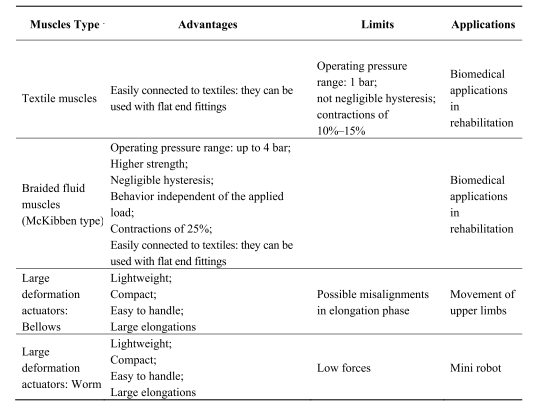
\includegraphics[width=1\textwidth]{Table_PAM_Features.png}
\end{table}

The first works on assistance to human lower limbs using soft robotics \cite{park2011bio,Hamedi2015} describe a soft orthosis for the foot intended to treat gait pathologies, particularly the drop-foot condition. One important aspect of this device is its design, inspired in the musculoskeletal human system, i.e. the actuation system was designed to comply a muscle-tendon-ligament functionality mimicking the natural behaviour of the human body (\autoref{fig:bio_ankle}). The soft orthoses is powered by pneumatic actuators, also called Mckibben-type actuators. They are attached to a soft support structure consisting of an adapted neoprene knee sleeve and a five toed leather shoe. A total of three off-the-shelf pneumatic muscles \autoref{fig:bio_ankle_parts}(a) assisted the dorsiflexion, eversion and inversion movements of the ankle joint by generating tension forces in artificial tendons, made of a flexible but non-extensible metal cable, positioned close to the foot tendons. The tendons were located inside a low friction material tube to prevent generated force losses; two of them were anchored to a single point in the foot brace while the other one was anchored in four different points in order to distribute the pulling force, again, mimicking the human body behaviour. The artificial ligaments provided with the same functionality as the biological ones, which is to restrict the movement of the tendons in all the directions other than the one of actuation (\autoref{fig:bio_ankle_parts}(b)). The pneumatic actuators were strategically anchored in two points, at the bottom of the knee sleeve providing nonrestrictive motion of the knee, and at the foot brace.
\begin{figure}[hbtp!]
    \centering
    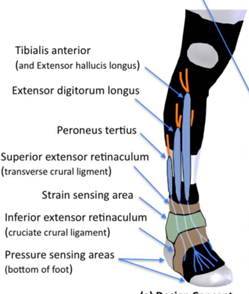
\includegraphics[width=0.4\textwidth]{BioinspiredAnkle.png}
    \caption{Design concept of the bio-inspired active soft orthosis for ankle foot. From top to bottom, the main parts are highlighted: artificial muscles attached to the soft wearable garment, a strain sensor for ankle angle measurements, the tendon-ligament system and pressure sensor for gait cycle detection \cite{park2011bio}. }
    \label{fig:bio_ankle}
\end{figure}
\begin{figure}[hbtp!]
    \centering
    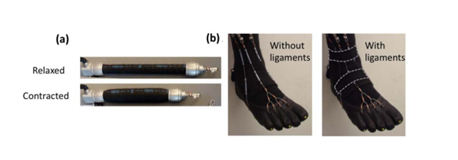
\includegraphics[width=\textwidth]{BioinspiredAnkleParts.png}
    \caption{Some components implemented in the soft orthosis, (a) pneumatic artificial muscle in its relaxed and contracted state and. (b) complete tendon-ligament system without ligaments and with ligaments. \cite{park2011bio}. }
    \label{fig:bio_ankle_parts}
\end{figure}

Another soft orthosis using pneumatic actuation is presented in \cite{Park2012} which extends the concept of embedded sensor and create an embedded sensor-actuator module, which is referred to as a muscle-sensor unit. In order to obtain some degree of compliance with human's lower limb, the device has a cylindrical shape and it is made of a flexible silicone elastomer (EcoFlex 0300). The muscle-sensor units are embedded into the latter shape to form a distributed array of four columns and four rows (16 actuators), allowing the device to have plenty of different motions and delivered torques depending on the number of activated actuators at a given time (\autoref{fig:soft_sleeve}). During the casting process, each column of actuators is tied to each other with Kevlar fibres so they can pull each other when contracting, also the fibres are anchored to both caps of the cylinder in order to achieve the desired movement. When the pneumatic muscle is activated its radius increases and its length decreases, creating a compression force. This design provides some degree of modularity due to the many embedded actuators which can be activated independently. Nevertheless, it has little compliance with the human's lower limb which ultimately complicates the conversion of generated forces into useful torques for assisting the joint of interest.
\begin{figure}[hbtp!]
    \centering
    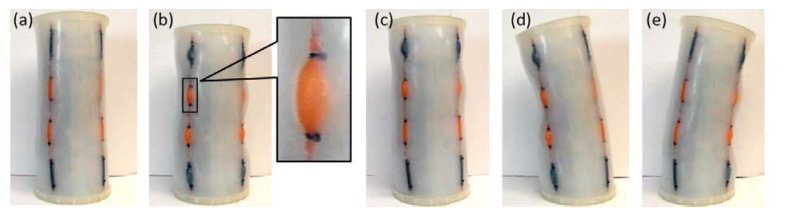
\includegraphics[width=\textwidth]{SoftSleeve.png}
    \caption{Different shapes achieved by the prototype. (a) Original shape. (b) All muscles activated, contracting the whole body and amplified image of one muscle. (c) Partial contraction, only the 1st and 2nd top rows are activated. Both (d) and (e) illustrate bending movements, only two adjacent columns are activated. \cite{Park2012}. }
    \label{fig:soft_sleeve}
\end{figure}

On the other hand, a novel implementation called virtual anchor technique, which used pneumatic artificial muscles, can be seen in \cite{wehner2013lightweight}. Addressing the challenge of force transmission using soft materials attached or strapped to the skin, which for high forces (such as those required in normal walking) will be intolerable for the user, the key anchor points of the human body are defined as the ones exhibiting large bony landmarks. These regions are able to withstand high forces and minimize the slippage or chaffing of soft materials positioning on them. Furthermore, the virtual anchor technique was also motivated by the changes in length of some parts of the skin surface during joint motion in where some parts exhibit more changes than others. Therefore, the soft exosuit was developed by interconnecting PMAs and nylon straps, replicating the extensible and non-extensible paths of the skin, respectively, in the specific points where the changes in the skin length take place, also called virtual anchor points which in combination with the key anchor points allow a good transmission of forces without causing discomfort to the user. In \autoref{fig:anchor_concept} the described concept can be appreciated, the orange lines represent the pneumatic actuators interconnected with the key anchors and the virtual anchors. The latter constrain the actuator's movements other than the desired, as well as redirect the actuator's reaction forces to the body areas able to sustain them. Finally, this design was able to reduce the metabolic cost caused by wearing the complete device of about 10 kg, by almost 100\%. Considering that no control system, other than a timed activation sequence, and no perception system was implemented, this technique opens the door for further improvements to achieve a better degree of assistance.

\begin{figure}[hbtp!]
    \centering
    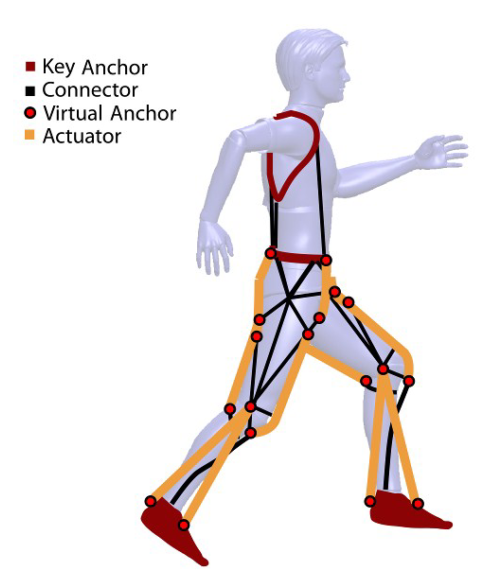
\includegraphics[width=0.45\textwidth]{AnchorConcept.png}
    \caption{Virtual anchor concept. The three key anchors (red square) located at the foot, hip and shoulder are interconnected with the soft actuators (orange) and auxiliary connectors (black) in specific points called virtual anchors (red circle) to stabilize the forces created by the actuators. \cite{wehner2013lightweight}. }
    \label{fig:anchor_concept}
\end{figure}

Putting aside the McKibben-type actuators as the most common choice for pneumatic muscles, elastomers such as high-flexible silicone can be used to build PAM as shown in \cite{Park2014}. This PAM consists of interconnected flat chambers made of silicone rubber which inflate when pressurized air is injected (\autoref{fig:Flat_elastomer}), the innovative concept in this work is the zero-volume air chamber which provides a higher degree of compliance and compactness (traditional PMAs retain air inside them even when they are not actuated). Kevlar fibres are embedded inside this soft actuator to constrain the expansion direction and create a contraction movement when pressurized. The flatness of this actuators simplifies the casting process. Furthermore, the chamber based design make it possible to join each chamber together not only in series, which increases the contraction length, but in parallel as well to increase the contraction force. In order to test the actuator performance, a soft exosuit similar to the previously described was developed using nylon straps and hooks to connect the soft actuator to the points of interest. The developed soft orthosis, intended for infant-toddler rehabilitation, was able to deliver a 38 N contraction force and 18 mm contraction length by implementing a muscle with an array of four elastomer actuators inter-connected in series. In addition, a total excursion for the knee joint of 132\textdegree{} was achieved, considering both flexion and extension motions (\autoref{fig:Flat_elastomer}). Moreover, in a most recent development by \cite{Low2016}, it can be found the implementation of elastomers for ankle assistance, in this case the pulling force of the PAM is generated when the actuator deflates and a pushing force is generated when it inflates, an inverted behaviour in comparison to previously mentioned applications. This soft orthosis consists of a regular sock which is attached to both ends of the PAM, that is enclosed into textile to restrict its longitudinal and radial expansion mainly. Despite the simplicity and assistance capabilities of the device, it can't be worn with shoes, restricting the assistance to indoor activities
\begin{figure}[hbtp!]
    \centering
    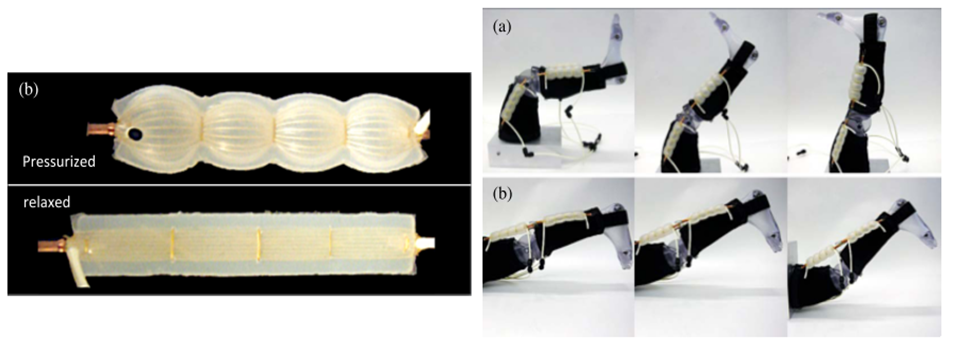
\includegraphics[width=1\textwidth]{FlatElastomer.png}
    \caption{(a) Flat elastomer pneumatic actuator in its both (1) pressurized and (2) relaxed states. (b) Implementation of the flat actuator in medical leg model assistance, along with the achieved extension (1) and flexion (2) motion. \cite{Park2014} }
    \label{fig:Flat_elastomer}
\end{figure}

This concept of expanding, instead of contracting, the PAM when pressurizing is called Inverse PAM (IPAM). This very recent type soft actuator, called `Hydro Muscle', is directly compared with McKibben muscles since it overcomes the main limitations of the latter. The main difference between this actuator and the previously mentioned is the shift from pneumatic technology to hydraulics, in fact, it is reported that the pressure found in homes tap water is enough to actuate it \cite{Sridar2016}. Therefore, the cylindrical shape `Hydro Muscle' is capable of elongating axially, increasing its stiffness radially, when pressurized; and of the exact opposite behaviour when depressurized (\autoref{fig:IPAM}). The actuator functionality is due to two structural layers of different materials. The inner layer is a tube made of an elastic material (latex showed better performance than the commonly used silicon) and the outer layer is made of a soft but inelastic material, such as polyester, which restricts the inner layer radial expansion and allows its axial expansion. Despite the simplicity of the design, this new concept of actuator is free of energy losses in radial expansion. Also, the energy losses inherent when using compressed air as the power source are not present in this design (in comparison to PAMs).
\begin{figure}[hbtp!]
    \centering
    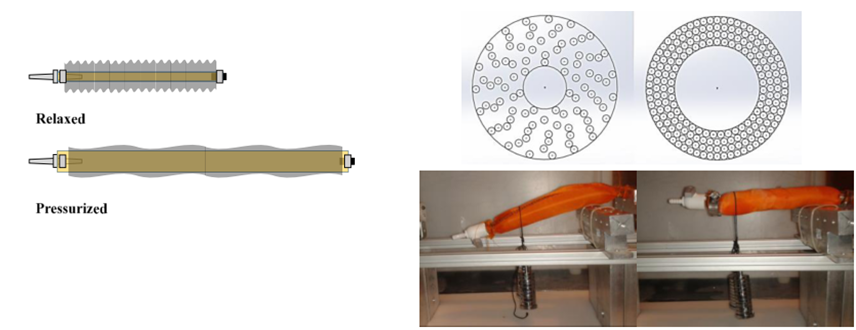
\includegraphics[width=\textwidth]{IPAM.png}
    \caption{a) Illustration IPAM developed in its relaxed and pressurized state, the small radial expansion and large axial expansion is appreciated. b) Cross-sectional view of the jamming effect ongoing inside the actuator (top), and bending effect (bottom) caused by heavy load, left hand side image, and correction of the bending using the jamming effect, right hand side image. \cite{Sridar2016}. }
    \label{fig:IPAM}
\end{figure}

The experiments performed in the paper showed that this innovative soft actuator is 33\% more efficient in comparison to a McKibben muscle using hydraulics. Furthermore, this actuator can be easily manufactured with off-the-shelf components. On the other hand, the convenience of using both pneumatic and hydraulic muscles for performing pulling instead of pushing tasks, is to prevent the bending effect caused when the actuator is fixed in one of its ends and has a heavy load attached to the other end. The latter effect is amplified for pushing tasks being one of the main drawbacks of the proposed actuator concept. However, a proposed solution is to use the principle of jamming by filling the gap between the inner and outer layer with granular media which will jam when the actuator is pressurized (\autoref{fig:IPAM}). Another IPAM development can be found in \cite{Hawkes2016} which implemented a very similar concept as the previously mentioned, however, this IPAM managed to achieve a strain of 300\% the length of the developed actuator whilst the previously mentioned IPAM only achieved a 100\% strain. The improvement in the achievable strain was mainly to the complete restriction of the stretchable material in the inner layer to only expand along its axis and not radially. Furthermore, the main benefits of IPAM in comparison with PAM are reported as follows: high strain and nearly linear control (since no radial deformation is present). The ability to achieve high strains make these soft actuators suitable for joints like the elbow.

\subsubsection{Cable-driven Actuators} \label{sec:cable-driven}

Another actuation technology implemented in soft orthoses are the Bowden cables in combination with electrical motors. Following the same principle as pneumatic muscles, this technology relies on generating tensions along a cable which, with a right positioning along the human lower limb, can transmit torques to the human body. The work in \cite{asbeck2013biologically} presents the design and implementation of a battery operated soft exosuit built with Bowden cables (\autoref{fig:bowden_exo}). 
\begin{figure}[hbtp!]
    \centering
    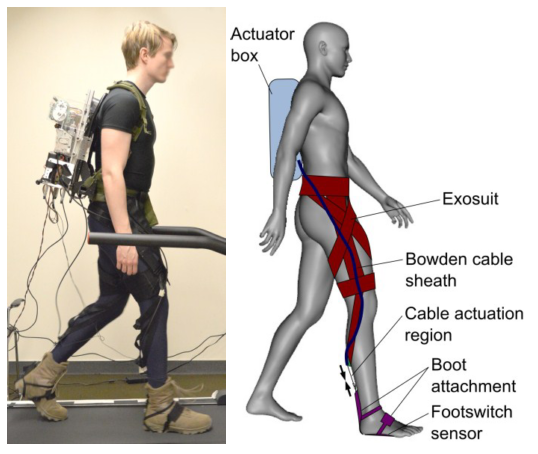
\includegraphics[width=0.5\textwidth]{BowdenExosuit.png}
    \caption{a) Developed Bowden cable-based soft exosuit prototype. b) Illustration of the initial design concept highlighting the main parts of the soft exosuit. \cite{asbeck2013biologically}. }
    \label{fig:bowden_exo}
\end{figure}

The exosuit is based on the leg's muscles functionality during normal walking, with the objective of assisting the forward propulsion stage of the gait. The soft exosuit structure made of fabrics is attached to the waist and above the knee, from the former the Bowden cable follows a path of webbing straps into the lower limb, ending at the ankle. In order to minimize the webbing strap structure chaffing and displacement when tensions are created along it, the strap along the waist of the user terminates at the hip since it is a bony part, i.e. there is almost no muscle and fat tissue between the skin and the bone, ultimately improving the exosuit stiffness. On the other hand, the suit delivers 18\% and 30\% of the torques required for normal walking on the knee and hip, respectively. However, despite the innovative design, the exosuit structure have limitations on the degree of compliance and stiffness, resulting in an approximately 13 cm displacement of the exosuit, when the Bowden cable is actuated. The biggest reported limitation during the experiment was the inefficiency of the Bowden cables, almost 45\% of the mechanical power generated by the actuator is lost, mainly in friction. However, the implemented multi-joint concept allows the actuation of two joints using a single actuator.

Following the multi-joint actuation concept, another soft exosuit is designed in \cite{Bartenbach2015} with the objective of not only providing assistance but also to enable impaired users. The concept (\autoref{fig:bowden_exo2}) exploits the benefits of using a single Bowden cable actuator to control more than one joint, multi-joint actuation. The difference in this case is the deep analysis performed regarding the compatibility of the joints, taking into account synergy of torque and equal polarity of torque, as well. In order to assist the desired movements of sit-to-stand, walking and stairs ascend, the knee and the hip joints were selected as the most suitable combination. Despite the fact the work was limited to describe the concept and design, by analyzing the selected joint combination it is expected to support the movements of sit-to-stand and stairs ascend.
\begin{figure}[hbtp!]
    \centering
    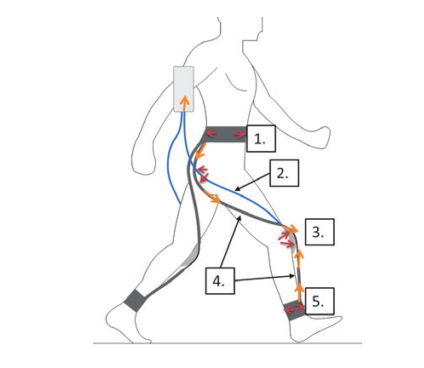
\includegraphics[width=0.7\textwidth]{BowdenExosuit2.png}
    \caption{Soft exosuit implementing the multi-joint actuation concept. A Bowden cable actuates the suit (2) by contracting the webbing element anchored at the hip (1) and shank (5). Reaction forces and actuation forces are represented in red and orange arrows respectively. \cite{Bartenbach2015}. }
    \label{fig:bowden_exo2}
\end{figure}

The next follow up on the concept of multi-joint actuation is documented in \cite{Ding2014} where a testing platform for soft exosuits was developed. The aim of this platform is to study the performance of the multi-joint actuation concept when being implemented in different soft exosuits. The off-board platform integrates the Bowden cable actuators and the sensors required to evaluate their performance. In addition, this platform can deploy sensors to be attached to the exosuit and compare relevant metrics such as mechanical power efficiency. This platform, which can be re-configurable to meet different applications, has been used to evaluate the advantages of implementing single joint and multi-joint actuation \cite{Ding2016}, highlighting the benefits of the latter. Furthermore, the study performed with the aid of this platform provided designing parameters for the development of an exosuit, in other words, the multi-joint platform assists the designing phase, ultimately reducing designing times.

\subsubsection{Shape Memory Materials}

The main two groups of shape memory materials implemented in soft robotics are: shape memory alloys (SMA) and shape memory polymers (SMP). Both technologies function under the same principle: they are able to switch into a different shape when a stimulus such as heat is in contact with them. Nevertheless, there are some differences to be mentioned. The SMA have to main phases, one for high temperature (austenite) and one for low temperature (martensite), when they suffer deformation while being in the martensite phase they can recover from the deformation by exposing them to heat, therefore SMA convert the energy from heat into mechanical energy to return to their original shape \cite{ImagesScientificInstrument2016}. This property is usually exploited to cause contraction changes in the mate-rial (\autoref{fig:SMA}). Therefore, SMA are commonly used in tendon-driven applications.
\begin{figure}[hbtp!]
    \centering
    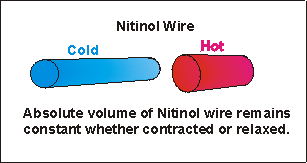
\includegraphics[width=0.5\textwidth]{SMA.png}
    \caption{Shape memory alloys made of Nitinol. The contraction effect under the increase in temperature is illustrated \cite{ImagesScientificInstrument2016} }
    \label{fig:SMA}
\end{figure}

The implementation of SMA into robotic applications have three main challenges to be addressed: response speed, high power consumption and low operational bandwidth. SMA make use of the Joule effect present in metals when an electric current flows through it, which generates heat. Depending on the metals used in the alloy, the amount of heat required for the SMA to recover from deformation is high enough to melt plastics, this excess of energy is what makes SMA inefficient \cite{Bundhoo2009a}. Furthermore, the large time required to cool down the SMA in order to repeat a cycle of deformation-recovery is another limitation which limits the operation frequency. This cooling process is usually performed by air convection which explains the large time (several seconds) required \cite{Bundhoo2009}. Therefore, SMA have been found to be unsuitable for orthoses or prostheses. However, plenty of authors have successfully developed the latter devices, in both rigid \cite{tarkesh2007} and soft variations \cite{Stirling2011}, capable of assisting human motions proving to be suitable for applications such as clinical rehabilitation where slow and repetitive cycles are required \cite{Pittaccio2009,Chenal2014}. Two comprehensive reviews documented in Pittaccio and Viscuso \cite{pittaccio2012shape} and Coral et al. \cite{Coral2012} illustrates the many other applications where SMAs are being implemented in the field of rehabilitation, such as: re-positioning, muscle toning, functional exercise and assistive robotics. Moreover, the review done by W. Coral \cite{Coral2012} also describes many works focused on addressing the SMA limitations.

The very interesting work done by J. Zhang in \cite{Zhang2013a} describes a SMA-based artificial muscle. This configuration facilitates the addition of a cooling system, due to the cylindrical hollow shape of the artificial muscle. Therefore, a mini pump is used to create a flow of air inside the artificial muscle which is able to reduce the cooling time by 10 times. The performance of this artificial muscle is further improved by taking into account the hysteresis behaviour typically found in SMA when shifting between the low and high temperature phases. Furthermore, there is again evidence of trying to replicate the muscle-tendon functionality, in this case by adding a spring in series with the artificial muscle which aids the SMA recovery phase and simulate a more realistic condition to the one at which the human muscles are subjected. The author is the first one able to model this behaviour and develop an adequate controller, which can be implemented in other scenarios involving SMA. Finally, this artificial muscle is implemented into an active foot orthosis (\autoref{fig:SMA_orthosis}) which achieves large contractile forces by using in parallel more than one SMA wire to form each of the pulling tendons. The main drawbacks were having low efficiency and low operational bandwidth.

\begin{figure}[hbtp!]
    \centering
    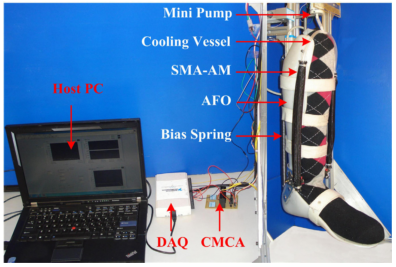
\includegraphics[width=0.7\textwidth]{SMAOrthosis.png}
    \caption{Developed soft orthosis for the ankle joint. The developed SMA artificial muscle along the main parts are highlighted. \cite{Zhang2013a}. }
    \label{fig:SMA_orthosis}
\end{figure}

Many attempts to improve SMA bandwidth have been made and since the theoretical bandwidth for a SMA is 3\% of its length, the most obvious approach is to increment the length of the SMA wire for a particular actuator but without increasing the length of the actual actuators. The latter can be achieved by using pulleys on each end-point of the actuator to develop, which allows the SMA wire to effectively increase its length without increasing the actuator length. However, implementing solely pulleys in a soft actuator greatly reduce compliance, increase the actuator weight and may cause twisting between the individual turns of the SMA wire. Therefore, a new approach described in \cite{Villoslada2015} proposes the implementation of Bowden cables outer sheath to contain the SMA wires inside. This concept allows the SMA to be directed in many ways to the point of interest, allowing the actuator to have different shape that can be compliant with the user's body, e.g. the SMA can be wrapped around the user's arm in a solenoid-like shape which also increases the SMA wire length (\autoref{fig:flexible_actuator}). Furthermore, pulleys are also implemented to allow the SMA to have a maximum number of three turns contained inside the Bowden sheath. Two main drawbacks were discovered during an experimental testing: SMA wires were twisting between each other which caused high friction losses and prevented the SMA to recover its initial length completely; the other drawback was the Bowden sheath material which was found to have low force transmission efficiency. In order to solve the latter, the Bowden cable sheath made of nylon was replaced by flexible tubes of Polytetrafluoroethylene (PTFE) and every SMA wire turn was individually encased in a narrow-gauge sheath. The final experiments showed that the developed actuator is able to contract 9\% of its length which is three times the theoretical contraction length of an SMA wire.

\begin{figure}[hbtp!]
    \centering
    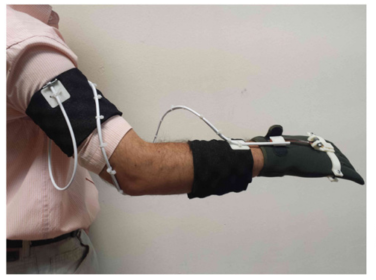
\includegraphics[width=0.5\textwidth]{FlexibleActuator.png}
    \caption{Flexible actuator around the arm in a wrist exoskeleton prototype. \cite{Villoslada2015}. }
    \label{fig:flexible_actuator}
\end{figure}

Shape memory polymers (SMP) are a little bit more complex than SMA. They have two main phases: a glassy state (high stiffness) and a rubbery state (low stiffness). Furthermore, when they are in their rubbery state, they can be deformed by applying small forces and preserve the deformation by cooling the SMP. In this state, the SMP can be considered rigid and it has to be heated to the point of the transition temperature to return to its original shape, hence having shape memory. This property of preserving a deformation is analyzed by K. Takashima et al. \cite{Takashima2010} in an attempt to boost the McKibben artificial muscle performance. McKibben actuators are unable to maintain their contraction shape unless precise and continuous control is implemented which cause premature wear on controlling elements as well as increase energy consumption. Therefore, a SMP is embedded into the McKibben braid which, by controlling the SMP temperature, allows the artificial muscle to hold its contracted position as illustrated in \autoref{fig:mckibben}. It is worth mentioning that SMP can be stimulating in different ways to obtain the change of shape, such as infrared light, electric field, magnetic field and even manipulating the material water content. In this work, the SMP made use of a heating source as well as compressor which drastically limited the developed actuator portability, but as previously mentioned, different stimulus sources can be used for different SMP.

The positive factors when comparing a SMA with a SMP are described, being the SMP benefits: light weight, low cost, rigidity in low temperature and flexibility in high temperature, higher strains, hence length deformation (around 400\% in comparison with 7\% for SMAs) and 3D shapes can be easily created. Furthermore, the main positive aspects of the improved McKibben are: allows rigidity fixing, the parameter to control stiffness can be used to control actuation and controllability of the actuator surface by individually stimulating certain segments of the SMP.

\begin{figure}[hbtp!]
    \centering
    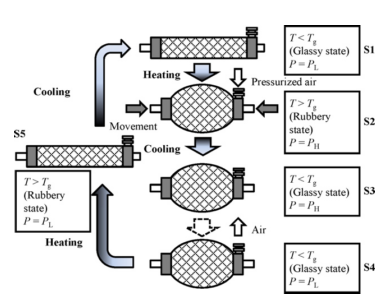
\includegraphics[width=0.8\textwidth]{Mckibben.png}
    \caption{Schematic illustrating McKibben with embedded SMP functionality \cite{Takashima2010}. $T_g$: transition temperature, $P_H$: high pressure, $P_L$: low pressure. }
    \label{fig:mckibben}
\end{figure}

\subsection{Soft Perception Technologies}
\subsubsection{Liquid metal alloys embedded into elastomers}

Strain soft sensors made of liquid metal alloys embedded into soft materials are being implemented into soft orthoses, such as the one in \cite{park2011bio}. The materials used in this case were Eutectic Gallium Indium (eGaIn), as the liquid metal alloy and flexible silicon rubber layer, which creates a really flexible sensor (\autoref{fig:strain_sensor}). The sensor was implemented to measure changes in the ankle joint proportional to the skin strain which it was attached to, by measuring the changes in resistance caused by the variations in the path length and cross-sectional area of the channel containing the liquid metal. Nevertheless, the developed soft orthosis implemented two other non-soft sensors: an inertial measurement unit (IMU) as an angle position detection and a pressure sensor attached to the shoe insole to detect foot strikes, hence the gait cycle. The developed strain sensor delivered good performance and contributed in the development of a feedback controller for this soft orthosis.

\begin{figure}[hbtp!]
    \centering
    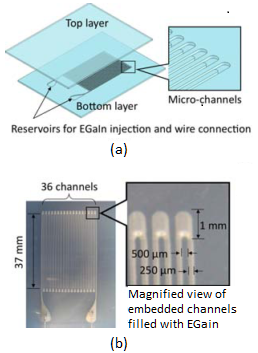
\includegraphics[width=0.6\textwidth]{StrainSensor.png}
    \caption{Soft strain sensor. The microchannel filled with liquid metal can be appreciated in: a) concept design and b) the prototype. \cite{park2011bio}. }
    \label{fig:strain_sensor}
\end{figure}

Liquid metal alloys are also implemented in \cite{Park2012}, as previously described, in the form of embedded muscle-sensor units (\autoref{fig:soft_sleeve_sensor}). The soft strain sensor was able to estimate the contraction length of a pneumatic muscle by measuring its radial expansion. In order to preserve softness, thin flexible copper wires were embedded into the cylindrical soft orthosis to obtain the sensor readings.

\begin{figure}[hbtp!]
    \centering
    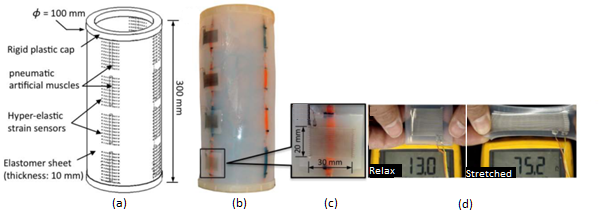
\includegraphics[width=0.9\textwidth]{SoftSleeveSensor.png}
    \caption{a) Design concept. b) Developed prototype. c) Magnified view of the embedded sensor-actuator concept. d) Soft strain sensor change in resistance during stretch. \cite{Park2012}. }
    \label{fig:soft_sleeve_sensor}
\end{figure}

Taking a step further the application of soft strain sensors with eGaIn, in \cite{mengucc2013soft} is presented in a wearable soft suit capable of sensing the joint angles of the hip, knee and ankle joints (\autoref{fig:Sensing_suit}). With the sensors properly positioned along the lower limb, by measuring the strain caused by the joint rotation, the join angle can be known. The sensors were able to track motions with a mean absolute error of 8\textdegree{}, being the most precise tracking achieved on the hip joint and the less precise on the ankle joint. In the mentioned work, only sagital plane motions were measured, however, due to the great success and linearity of the sensors, they are planned to be implemented to measure motions in the frontal plane as well. The complete suit characterization can be found in \cite{mengucc2014wearable}.

\begin{figure}[hbtp!]
    \centering
    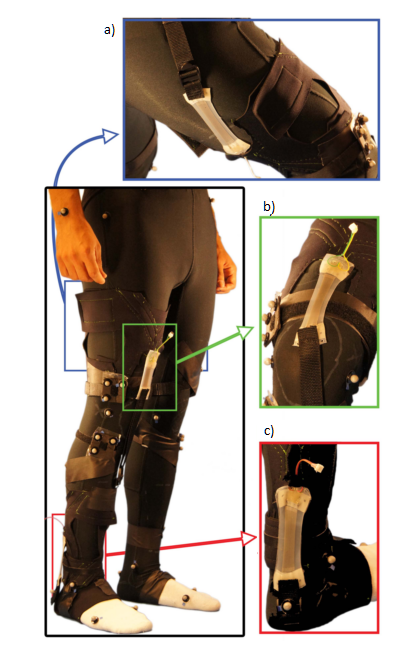
\includegraphics[width=0.4\textwidth]{SensingSuit.png}
    \caption{Implementation of soft strain sensors into a Soft sensing suit, from top to bottom: hip sensor, knee sensor and ankle sensor position. \cite{mengucc2013soft}. }
    \label{fig:Sensing_suit}
\end{figure}

On the other hand, a potentially improved version of these soft strain sensors is presented in \cite{Chossat2013} where the highly stretchable elastomer is filled with two different conductive liquids, a traditional liquid metal and an ionic solution, instead of one. Interconnecting the strain soft sensor with the external application has been a big challenge, since the strain caused by the connection, usually soft wires, affects the sensor accuracy by increasing the total electrical resistance and by generating additional strain. Nevertheless, the ionic solution is intended to decouple the signal routing part from the sensing part in order to solve the latter challenge, creating a noise-free interface with the external application (\autoref{fig:hybrid_strain_sensor}).

\begin{figure}[hbtp!]
    \centering
    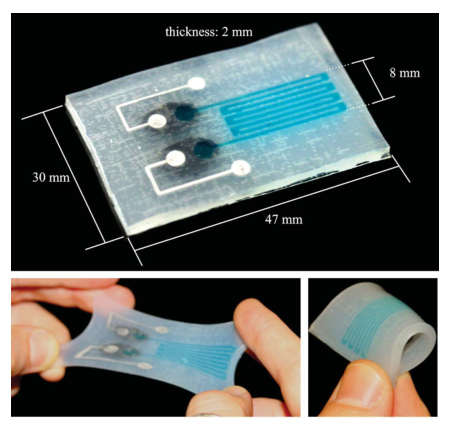
\includegraphics[width=0.5\textwidth]{HybridStrainSensor.png}
    \caption{Hybrid soft strain sensor, the interface between the liquid metal and the ionic solution can be clearly seen in dark areas. \cite{Chossat2013}. }
    \label{fig:hybrid_strain_sensor}
\end{figure}

One direct implementation of the embedded microchannel with conductive fluid sensors, can be seen in a recent improvement to the McKibben type PAM (\autoref{fig:braided_sensor}). McKibben actuators were strongly adopted in soft robotics applications and there is plenty of information in the literature about their implementations, modelling, etc. However, accurately sensing these actuators parameters such as deformation and force when they are pressurized was still a challenge being addressed in many forms such as: cylindrical dielectric elastomers with carbon grease disposed on their surface to function as electrodes \cite{Goulbourne2007}; and attaching to the actuator an elastomer sheath with microchannels filled with conductive fluid which surround the actuator in a helical shape \cite{Park2013}. Both the microchannels and the electrodes represent a resistor which will change its physical dimensions, by extension its electrical resistance, when the actuators compress or stretch which provides a measure of the actuator deformation. Furthermore, the idea of a helical path surrounding the actuator was extended to a solenoid shape and to the so called 16 helices shape, as shown in \cite{Felt2014,Felt2015}. From the electric circuit created, it is possible to measure both the output force and length deformation of the actuator by correlating them with the circuit resistance and inductance respectively. This work proposed the implementation of conductive wires to build the reinforced braid of a McKibben actuator allowing the actuator to `sense', from there the given name of `Smart Braid', creating a solenoid like circuit from which the inductance can be measured using a couple of mathematical approximations such as: the Neumann approximation (for the 16 helices shapes) and the long solenoid approximation, being the former one the most accurate and general; but at the same time the most expensive in terms of computation. The author exerts that this new sensing concept can be applied to multitude of scenarios in soft robotics, which includes soft orthosis.

\begin{figure}[hbtp!]
    \centering
    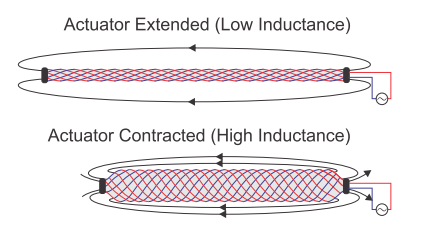
\includegraphics[width=0.5\textwidth]{BraidedSensor.png}
    \caption{`Smart Braid' concept. The variation in the actuator length cause a change in the electric circuit inductance. \cite{Felt2015}. }
    \label{fig:braided_sensor}
\end{figure}

\subsection{Control Technologies} \label{sec:controlSystems}

One of the successfully implemented control systems is documented in \cite{park2011bio}, which is the ankle soft orthosis previously mentioned. The control system is comprised of several micro-controllers for parallel processing, and is divided into four main stages: sensing, signal processing, control and actuation (\autoref{fig:control_system}). The soft orthosis makes use of three different sensor technologies which requires different sampling and signal processing algorithms for each one, the IMU being the most complex one. Thereafter, another micro-controller with access to all the sensors, makes the decision to activate the solenoid valves that control the pneumatic muscles by generating a pulse width modulating (PWM) signals which in combination with binary on/off valves are able to perform a proportional control type. No mathematical model was deducted to describe the non-linear behaviour of the pneumatic muscles, instead, simpler controller approaches as feed forward and feedback controller were being implemented, with the latter being able to achieve a response time of 500 ms when a perturbation was present on the system, such as letting a weight hang from the device toe. The feedback controller made use of a soft strain sensor (previously mentioned) to correct the ankle angle. Finally, although the controller performance is good it is still not enough to provide active gait assistance nor to predict user intentions. Another drawback, minor in this case, is that the system requires calibration every time a new user wears it. Nevertheless, the developed soft orthosis is suitable for rehabilitation because it can achieve a dorsiflexion of 12\textdegree{} and 20\textdegree{} when foot was at resting position, and when foot was forced to a plantarflexion position, respectively; in addition, the perception system could provide the clinician with meaningful data about the patient progress. The previous work was continued in \cite{park2014design} where a new controller was designed by considering the interaction between the soft exosuit and the human body as a black box, i.e. instead of trying to model the non-linear behaviour of the whole system some experiments were performed to obtain a system input/output relationship and after that implement classic control techniques to model a linear time invariant controller. The results were promising since the original complex system was able to perform accurately using simple techniques. Finally, the addition of electromyography sensors was discussed to add the involuntary muscle contractions of the user into the system as a disturbance and improve the accuracy during different scenarios.

\begin{figure}[hbtp!]
    \centering
    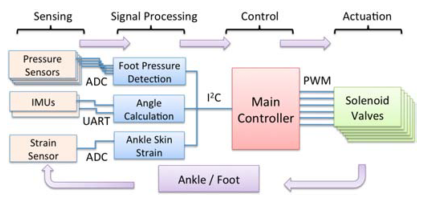
\includegraphics[width=0.7\textwidth]{ControlSystem.png}
    \caption{Control system architecture implemented for the ankle soft orthosis. \cite{park2011bio}. }
    \label{fig:control_system}
\end{figure}

In some cases, the design and development complexity of a controller for soft devices restrain the research extend to focus only on the implementation and study of soft actuation and perception systems. This is the case in \cite{Park2012}, the cylindrical soft sleeve with embedded muscle-sensor units; where the developed controller is well designed but with no close-loop architecture nor complex mathematical model to predict the soft material behaviour. Again, the controller system is integrated by several micro-controller units, each of those communicated with their surrounding neighbours, in fact, each of the 16 nodes embedded into the cylindrical soft sleeve has one. Furthermore, each controller architecture has two layers, one dedicated to the collection of sensor data, intercommunication between the micro-controller units, specify actuation parameters and schedule of tasks. The scheduler is implemented as a means to synchronize the otherwise independent micro-controller units and behave as a network, converting the system into a sequential one instead of a parallel one as previously mentioned. Every unit has four tasks to execute at a given time and a given order: sensing, communicate, process data and actuate. On the other hand, the actuation parameters are generated using a mathematical approximation of the soft material behaviour which assumes no deformation is caused by the compression of the pneumatic actuators, other than the length change present where the actuators are embedded, this means the diameter of the cylinder remains constant as well as the length in the other side of the cylinder. The experiment proved the requirement of a better approximation, since for a desired bending angle of 15\textdegree{}, an actual bending of 11.5\textdegree{} was achieved, and feeding the soft sensors data into the mathematical approximation, a bending of 13\textdegree{} was estimated; therefore, achieving an accuracy of 76\%.

The fact that few soft exosuit developments fully implement a controller system does not imply that no research is being performed in the field. The implementation of current soft actuators into functional devices, as well as the proof of concept of emerging soft actuators are usually followed by an extensive study about modelling their behaviour to translate that information into a controller system. Solely for PMAs several work has been done, even implementing fuzzy logic to achieve better results, in \cite{Chang2015,Skorina2015,Bishop-Moser2015,Hosovsky2016}. The next step in the research cycle of all the soft actuation technologies is to implement the tested models into functional devices, which then will allow new concepts to be developed, hence new modelling research to be performed.

\section{Gaps in the Body of Knowledge} \label{sec:gaps}

The available literature suggests a growing interest in the research and development of soft actuation technologies, soft perception systems, and control systems to pair with the latter two. Also, and following the bioinspiration driving the field of Soft Robotics, many works are attempting to imitate the capabilities of the human musculoskeletal system by developing soft actuator that behave like the human muscle-tendon component. This is more evident when looking at the available works on Pneumatic Artificial Muscles (PAMs) described in \autoref{sec:PMAs}, where an actuator is used as the contractile force generator element (muscle), and a flexible interface (tendon) is used to transmit that force to the desired location. Similarly, established technologies such as electric motors, which are able to deliver forces in both directions of rotation, are being used in combination with Bowden cable to create pulling forces, as mentioned in \autoref{sec:cable-driven}. This type of setup is known as a redundant system because more than one actuator is required to control both directions of rotation of a joint. Moreover, the research and development of new soft materials, such as the SMA and SMP, is also focused on creating materials able to contract when stimulated. There is still plenty of work to be done in this matter, which is why this is identified as one gap in the body of knowledge.

The vast majority of available literature is focused on testing a new soft actuation concept in an open-loop approach, i.e. with no control system implemented. This is caused by the fact that modelling the mechanical behaviour of a soft material is very complex. Even the control system of the most documented work in the literature, the ankle-foot orthosis, does not implement a modelling technique to monitor the behaviour of the PMAs, instead it is focused on extracting as many information as possible from the environment and use this to decide when and how to activate the PMA \cite{park2011bio}. The scarce literature about the control systems of soft robotic applications, as evidenced in \autoref{sec:controlSystems} is identified as another gap in the body of knowledge.

Therefore, two main gaps are considered in the body of knowledge which are addressed by this research. On the one hand, there is still many work to do in understanding the functionality of the human musculoskeletal system, and in developing a soft actuation technology which mimics the functionality of the muscle-tendon component. On the other hand, there is a lack of reliable modelling tools to predict the complex mechanical behaviour of soft materials being used in soft actuation technologies. 

\section{Summary}

According to the literature, the most commonly implemented soft actuation technologies in soft robotic applications for human assistance are: Pneumatic/hydraulic artificial muscles, cable-driven actuators based on electric motors, and shape memory alloys/polymers.  In cable-driven actuators, the amount of generated assistance is proportional to the electric motor mechanical output power. This means, large forces can be generated to even enhance the user capabilities, yet again, the transmission of this forces via the human body prevents this enhancement. A common problem is the relative displacement of the soft structure worn by the user when tensile forces are generated by the pulling action of Bowden cables. Nevertheless, one advantage of this technology in soft exosuits is the `remote' actuation capability, which means that the electrical motors can be placed distal to the joint to be assisted, concentrating the weight of the heavy parts of the soft exosuit in convenient locations of the human body, e.g. as a backpack. Another advantage of this technology is the flexibility of the Bowden cables which allows them to be deployed in many different trajectories along the human body, facilitating the use of the body parts capable of sustaining high forces.

In contrast, the other two soft technologies are commonly placed proximal to the joint to be assisted, which might allow a better distribution of the soft orthosis weight. Recent works have tackled the main limitations of PAMs, SMA and SMP. Particularly, big improvements have been achieved for PAMs and SMA. For the case of PAMs, the traditional and extensively implemented McKibben type muscle have been improved in terms of performance by the development of the Inverse PAM (IPAM). This latter technology surpasses the McKibben type muscle in assistance capabilities, efficiency and controllability. Furthermore, the concept of the IPAM can also be implemented using hydraulics which again comes with several advantages, a crucial one, the amount of exerted force. The main disadvantage of both pneumatic and hydraulic actuators is the need for a compressor unit, which greatly decreases the soft orthosis autonomy and portability. Nevertheless, the recently developed `Hydro Muscle', which uses pressurized water from a home tap, greatly increases the appealing of this technology. In a similar way, the greater efficiency of IPAMs allows portable tanks with pressurized air to be used.

The situation is quite similar for SMAs, many of the limitations from this technology, such as low strain, slow speed response and complex controllability have been addressed and improved. However, this technology is still in its early stages and their main drawbacks, such as high energy consumption and being unsafe for human interactions applications due to the high levels of heat they reach, make them unsuitable to be deployed in real soft robotic applications.

In the field of soft sensors, one of the main advantages of the soft strain sensors is that they can be custom-built to fit any application. When characterizing these sensors, two parameters are always mentioned: the electrical resistance and the gauge factor, the latter relates the strain with the change in resistance. Despite their original purpose of measuring strain changes, they can be used for angle measurements. On the controller side, the amount of research being performed in modelling the complex behaviour of soft actuators is slowly but constantly increasing. Nevertheless, the complexity and time consuming of tackling the latter is evidenced in the scarce literature available.

In summary, this literature review highlighted a very specific and bioinspired trend in soft robotic applications for human assistance, which is mimicking the human musculoskeletal system, specifically the muscle-tendon component. This approach is very compatible with soft technologies that are commonly placed proximal to the assisted joint (PAMs, SMAs, IPAMs, etc.), and many soft artificial muscles have already been developed. These works, however, have mainly focused on the contractile element of the muscle-tendon component, leaving plenty of room to research about the viscoelastic element, the tendon. The most straightforward to study the potential benefits of mimicking the human tendon behaviour, is to incorporate soft materials, to current soft actuation technologies, as part of the mechanism to transmit the generated forces. Essentially, creating a soft artificial tendon. Nevertheless, the success of maturing the previous concept into a soft robotic application greatly depends on having a reliable modelling tool which predicts the mechanical behaviour of soft materials. Finally, as mentioned in \autoref{sec:gaps}, this research aims to address two main gaps in the body of knowledge. On the one hand, the lack of literature about the implementation of soft materials as part of the force transmitting mechanism, which could allow for a better mimicking of the human musculoskeletal system. On the other hand, the lack of a modelling tool able to predict the mechanical behaviour of soft materials.
